\section{Introduction}
\begin{quotation}
\textit{Imagine an earthquake has hit a populous area and many major roads are
impassable. Buildings are severely damaged or collapsed, and fire has broken out
in many places. At the crisis management center, response professionals are
working together to coordinate the earthquake relief effort. You are the
incident commander charged with coordinating the search
and rescue teams working in the field. There is a large tabletop display in
front of you, showing the map of the site. Information coming from the field is
updated on the display in real-time.}

\textit{A report about a big explosion at a chemical plant comes in and you move
the map around, zoom in and rotate it to get a good view of the plant. On the
map, you see there is a group of unmanned vehicles nearby. After selecting them
on the map with your hand, you speak to the interface ``Go nearer to the
explosion site to gather more information,'' while tracing the route the
vehicles should take to avoid obstacles. Then you instruct rescue team No. 3 to evacuate the residents
in the surrounding buildings by going under a bridge because the surface of the
bridge is blocked. You gesture with one hand as the bridge and the other
hand moving under it to emphasize this.}
\end{quotation}

The scenario above is an example in the Urban Search and Rescue (USAR) domain.
It shows an application of a multi-modal interface to a real-world problem. Gestures play an important part in this scenario,
providing key information about location, method and timing of movements,
and about spatial relationship among the objects being described.

Recent trends in user interfaces have brought on a new wave of interaction
techniques that depart from the traditional mouse and keyboard that have been 
used for decades. These include multi-touch interfaces such as the 
iPhone, the iPad and the Microsoft 
Surface\textsuperscript{\textregistered} as well as camera-based systems such as
the Microsoft Kinect and the Nintendo\textsuperscript{\textregistered} Wii. Most
of these devices gained instant popularity among consumers, and the common trait
among them is that they make interacting with computation more natural and 
effortless. All these devices allow users to use their hands and/or body 
gestures to directly manipulate the virtual objects. It feels more natural this 
way because this is how we interact with our environment in everyday life.
 
Our goal is to take this aspiration to the next level by developing an
intelligent multi-modal interface for natural interaction. By \textit{natural
interaction}, we mean the kind of cognitively transparent, effortless
multi-modal communication that can happen between people; we want to make this possible in
human-computer interaction such that the computer interface understands what the
user is saying and doing, and the user can simply behave. We believe that
natural interaction can provide better learnability, flexibility, memorability,
convenience and efficiency, but further user studies are needed to investigate
this belief.

Gesture plays an important part in multi-modal interaction, especially for
conveying spatial information. The focus of this thesis is developing a
hierarchical approach for continuous gesture analysis that can be easily
applied in different domains and applications. Specifically, we focus on
gestures made with hands. 

I propose to develop a gesture-based interface that allows users to perform
manipulative and communicative gestures continuously with no arbitrary
restrictions. The key elements of the approach are the hierarchical framework
for gestural analysis based on abstract hidden Markov models (AHMMs) and the
accurate real-time detection of the onset of natural gestures that convey 
information intended by the users, while filtering out movements that do not 
convey information.

\section{Background}
\subsection{Definition of Gestures}
Webster's Dictionary defines gestures as ``\ldots the use of motions of the
limbs or body as a mean of expression; a movement usually of the body or limbs
that expresses or emphasizes an idea, sentiment, or attitude.'' This definition
is particularly related to the communicational aspect of the human hand and body
movements. However, in the domain of human computer interaction (HCI) the notion
of gestures is somewhat different. In their review of the visual interpretation
of hand gestures for HCI, Pavlovic et al. \cite{Pavlovic97} states that in a computer
controlled environment one wants to use the human hand to perform tasks that
mimic both the natural use of the hand as a manipulator, and its use in
human-machine communication. They include both manipulative and communicative
gestures in their gesture taxonomy. This is also the definition we will use in
this thesis.

Pavlovic et al. \cite{Pavlovic97} also gives a model (Figure. 
\ref{fig:gesture_production}) for the production and perception of gestures 
based on the model used in the field of spoken language recognition. According 
to their model, gestures originate as a gesturer's mental concept, possibly in 
conjunction with speech. They are expressed through the motion of arms and 
hands. Also, observers perceive gestures as streams of visual images which they
interpret using their knowledge about those gestures. In HCI, the 
observer is the computer and the knowledge it possesses is the training data we 
give it.

\begin{figure}[h]
  \centering
  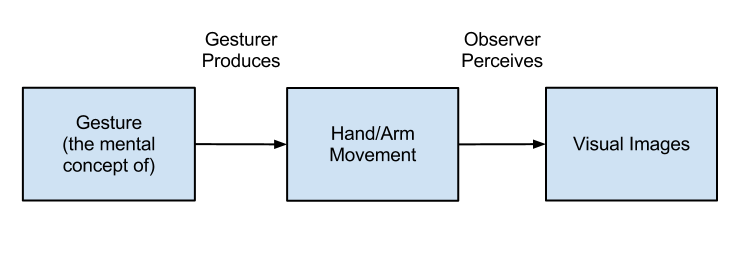
\includegraphics[width=0.7\textwidth]{figures/gesture_production.png} 
  \caption{Production and perception of gestures. Hand gestures originate as a
  mental concept, are expressed through arm and hand motion, and are perceived
  as visual images \cite{Pavlovic97}.}
  \label{fig:gesture_production}
\end{figure}

\subsection{Gestural Taxonomy}\label{sec:taxonomy}
The mental concept of a gesture represents the semantic meaning or the
actual intention of the gesturer. In this dimension, hand movements can be
divided into different general categories. Each category has its own characteristics and requires different responses from the computer interface. Having a systematic gesture taxonomy can inform
us about the design of the interactive system. The taxonomy will also be the
basis of our hierarchical approach to gesture interpretation. Our gesture
taxonomy (see Figure \ref{fig:taxonomy}) is based on the one developed by Pavlovic et al.
\cite{Pavlovic97} with some changes to make the terminology clearer. This is
also similar to the \textit{nature} dimension in the taxonomy proposed by
Wobbrock et al. \cite{wobbrock09}

\begin{figure}[h]
  \centering
  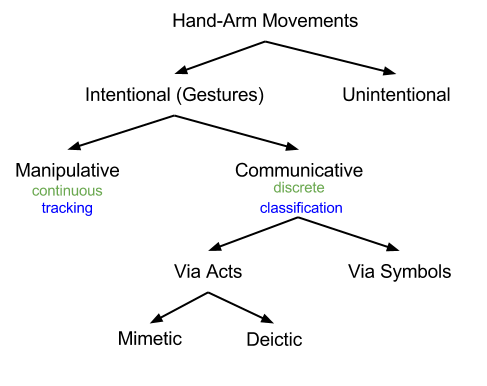
\includegraphics[width=0.5\textwidth]{figures/taxonomy.png} 
  \caption{Gesture taxonomy}
  \label{fig:taxonomy}
\end{figure}

First, gestures, as \textit{intentional} movements, should be distinguished from
\textit{unintentional} hand movements (like beats). By \textit{unintentional}
movements, we mean movements that are not intended to convey information. In
contrast, gestures are meaningful hand movements that people make to convey some
information. The distinction is important for a natural interface because there
should not be any restriction on how people should place or move their hands
when they are not doing any meaningful gestures. 

Gestures are then further divided into manipulative and communicative
categories. Manipulative gestures are used to act on objects (e.g.
moving an virtual object around, click a button, the property of the virtual
object change directly according to certain parameters of the hand(s)), while
communicative gestures have an inherent purpose for communication \cite{Pavlovic97}. For manipulative gestures, the system needs to respond frame by frame while the user is doing certain direct manipulations. This can be achieved by tracking the hand state in real-time. For communicative gestures, the system needs to respond to
the meaning of the gesture when the user finishes performing the gesture. This part is
accomplished by gesture recognition. So manipulative gestures and communicative
gestures fall into the \textit{continuous} category and the
\textit{discrete} category respectively in the \textit{flow} dimension of the
taxonomy proposed by Wobbrock \cite{wobbrock09} et al. based on their
user study.

People perform communicative gestures via acts or symbols. Gesture via acts are
those directly related to the interpretation of the movement itself. Such
movements are classified as either mimetic (which imitate some actions) or
deictic (pointing acts that convey spatial information). Gestures via symbols
are those that have a linguistic role, and are often represented by different static hand postures. An example is forming the
O.K. pose for ``accept''. 

The physical arm and hand movements that express the mental concept of the
gesture can be categorized into different \textit{forms} \cite{wobbrock09} as
shown in Table \ref{tab:form}. Both manipulative and communicative gestures can
have all of these forms. This means that the features we want to use for
gestural analysis should be based on both the hand pose and the locus of the
hand movement.

\begin{table}[h]
  \centering
  \begin{tabular}{| l | l |}
  	\hline
  	\textbf{Form} 		  & \textbf{Description} \\ \hline 
  	Static pose  		  & Hand pose is held in one location. \\ \hline
  	Dynamic pose 		  & Hand pose changes while location does not. \\ \hline
  	Static pose and path  & Hand pose is held as hand moves. \\ \hline
  	Dynamic pose and path & Hand pose changes as hand moves. \\ \hline
  \end{tabular}
  \caption{Different gesture forms.}
  \label{tab:form}
\end{table}

\subsection{Temporal Modeling of Gestures}
Since human gestures are a dynamic process, it is important to consider the
temporal characteristics of gestures. This may help in the temporal segmentation
of gestures from other unintentional hand/arm movements \cite{Pavlovic97}. It
has been established that three phases make a gesture:
\begin{itemize}
  \item preparation,
  \item nucleus (peak or stoke \cite{mcneill82}), and
  \item retraction \cite{Pavlovic97}.
\end{itemize}
The three temporal phases are distinguishable through the general hand/arm
motion: ``Preparation'' and ``retraction'' are characterized by the rapid change
in the position of the hand, while the ``nucleus'' or the ``stroke'', in
general, exhibits relatively slower hand motion. The ``stroke'' of a gesture, as
Kendon \cite{kendon86} observes, has some ``definite form and enhanced dynamic
qualities''. Every gesture must have a ``stroke'', which is considered by Kendon
to be the content-carrying part of the gesture. Based on this theory, we
expect that he lack of the ``stroke'' part is how unintentional movements can
be distinguished from gestures. However, Kendon does not explain exactly what
the dynamic qualities are. Hence, this is what this thesis is going to explore, i.e., what forms and dynamic qualities differentiate gestures from unintentional movements.

\section{Research Questions}
This thesis focuses on several research questions that aim to solve some of the
key challenges in developing a multi-modal interface with natural gesture input.

\begin{itemize}
  \item \textbf{Fine-grained hand pose estimation.} The hand model for
  gestural input can range from a very simplistic one (one point) to a very
  comprehensive one (a 26 degrees of freedom (DOF) skeleton). There is a trade
  off between the accuracy of the model and computational complexity. The question
  here is what hand model is sufficient for the HCI tasks for both manipulative
  and communicative gestures.
  \item \textbf{Online gesture spotting.} A real-time gesture-driven HCI
  application requires gesture spotting with minimum delay. The questions are how to accurately determine the
  start and the end of a gesture in real-time, and how to filter out
  unintentional hand movement.
  \item \textbf{Unified hierarchical model for gestural analysis.} We propose a
  unified framework based on AHMMs that distinguishes unintentional movement,
  manipulative gestures and communicative gesture in real-time and provides
  appropriate responses to the user.
\end{itemize}

\section{Related Work}
There is a large body of active research on using the hand as an input modality
for human-computer interaction. To do this, the computer needs to be able to
interpret the dynamic and/or static configurations of the human hand, arm, and
even other parts of the human body. We break down the gestural input
system into several sequential modules shown in Figure \ref{fig:pipeline}.

\begin{figure}[h]
  \centering
  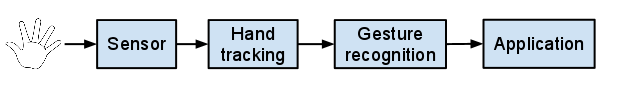
\includegraphics[width=0.7\textwidth]{figures/pipeline.png} 
  \caption{Gestural input pipeline.}
  \label{fig:pipeline}
\end{figure}

\subsection{Sensors}
The first step in the pipeline is having sensors that capture the hand movements
and configurations, converting analog signals to digital signals. First attempts
to solve this problem resulted in mechanical devices that directly measure hand
joint angles and spatial positions. This group is best represented by the
glove-based approaches using devices such us CyberGloves \cite{fels09} and
Powergloves \cite{kadous02}. However, wearing gloves makes gesturing more
cumbersome, and many efforts have been made to make the gloves more
light-weight, for example, by using Bluetooth wireless data transmission (e.g.,
CyberGove II). To further reduce the bulkiness of the gloves, people use colored
markers on the fingers \cite{mistry09} or colored gloves with no electronics \cite{Wang09}, and use RGB
cameras and computer vision techniques to interpret gestures. However, by
requiring the user to wear something extra still hinders the acceptance of
such devices as ``everyday'' natural interaction interfaces. 

The most non-obtrusive way to capture the hand is bare-hand tracking. Shin et
al. \cite{Shin04} use stereo RGB cameras to extract the hand from background based on the skin color. One
limitation of RGB cameras is that they are very sensitive to lighting
conditions. This prompted researchers to look into other types of cameras. Oka et al. 
\cite{Oka02} use thermal imaging for hand segmentation under complex
background and changing light, relying on the condition that a hand's
temperature is almost always distinct from the background. Their approach does
not detect finger contact with the surface. Larson et al. \cite{larson11}
improve on this method to detect the finger contact by using
the heat transferred from a user's hand to the surface for touch-based gestures.
However, in order to detect the heat trace, the user has to drag the fingers a
bit instead of just touching. This may be a small departure from what users
would expect as ``natural'' based on their experience in the physical world.

Thermal imaging measures radiation emitted by objects in the
\textit{far}-infrared (F-IR) spectrum. There are other well-known ``IR-imaging''
techniques used in the HCI community which use devices that operate in the \textit{near}-infrared (N-IR) spectrum.
N-IR is employed in some fairly recent interactive tabletop surfaces and depth
cameras. A number of projects in the HCI community have used IR for tabletop
interaction by detecting multi-touch gestures using an under mounted
camera and an illumination source. An example of this is Microsoft's 
Surface\textsuperscript{\textregistered}. Recently, portable multi-touch devices
such as phones and tablets have become more and more ubiquitous. These devices
are based on capacitive touch sensitive screens. Touch-based devices are
becoming more and more mature, however the kind of gestures one can use are still
limited. The gestures are usually limited in 2D space with one or multiple
fingers. 

Going beyond the limitation of touch-only gestures, researchers at Microsoft
augmented the Surface technology with a switchable diffuser, additional
strips of IR LEDS with a different wave length for diffuse illumination, and an
additional IR sensitive camera which images IR reflected from the diffuse
illumination of the environment \cite{hilliges09}. In this way, they can capture
the hand above the surface as well. The height of the hand is estimated based on
the pixel intensity.

Since the introduction of Kinect, a motion sensing input device by Microsoft for
the Xbox 360 video game console, researchers in the HCI community, as well as
many independent hackers, have been using Kinect's depth sensor for capturing
both body and hand gestures \cite{openni}. Since then, there are also many
similar devices coming into the market which have been used for capturing
gestures. For instance, Harrison et al. \cite{harrison11} use  a short-range
PrimeSense \cite{primesense} depth camera for their wearable multi-touch
interaction. In comparison to the aforementioned augmented Surface setup,
Kinect, and the likes, provide a cheap alternative for depth sensing. In this
thesis, we will explore the potential of using the Kinect sensor for detecting 
both the touch-based gesture and above-surface 3D gestures. Potentially, we can 
use the depth information for determining surface touch, and hence, eliminate
the need for the complicated electronics of a touch sensitive screen. This also 
enables the gestural interaction on a large tabletop display, much bigger than 
that of Microsoft's Surface.

\subsection{Hand Tracking}
After getting input from the sensor(s), the next step in the pipeline is
tracking the hand(s). This is essentially the frame-by-frame estimation of the
parameters of the hand model based on the sensor input. The complexity of the
hand model is application dependent. For a given application, a very coarse and
simple model may be sufficient. The simplest model is treating the hand as a
blob and only the 2D/3D location of the blob is tracked. For example, Sharma et
al. \cite{sharma00} use 2D positional and time differential parameters to track
the hands as blobs, which is sufficient for them to distinguish whether the
hands are doing a point, a contour, or a circle gesture. The PrimeSense NITE
middleware for OpenNI's natural interaction framework also tracks the hand as a
point. It requires the user to do a ``focus'' gesture (``click'' or ``wave'')
to gain control in order to start hand tracking \cite{primesense-manual}. The
gestures it supports are ``click'', ``wave'', ``swipe left'', ``swipe right'', 
``raise hand candidate'' and ``hand candidate moved''.

However, to make a more generalizable system for natural-like interaction, a
more sophisticated model is required. One step forward is adding fingertip
locations in the hand model as exemplified in \cite{Oka02} \cite{harrison11}
\cite{larson11}. Tracking fingertips is usually sufficient for manipulating
objects on the 2D surface. However, for a more rich set of gestures, the one
that also involves communicative gestures, we may need a more sophisticated
model. For instance, Wang et al. \cite{Wang09} uses a 26 DOF
3D skeletal model in their real-time hand-tracking system. 

Another approach is using an appearance-based model. This means that the model
parameters are not directly derived from the 3D spatial description of the hand.
The hand poses are modeled by relating the appearance of any pose to the 
appearance of the set of predefined, template poses \cite{Pavlovic97}. In
their markless hand-tracking system, Wang et al. \cite{wang11} use efficient
queries of a database of gestures and desktop-specific hand silhouette samples
for pinch/click gesture detection.

In our system, we propose a combination of both approaches. A simplified 3-D
skeletal hand model is useful for manipulative gestures because we want to know 
exactly where the fingertips are and the grabbing and releasing poses of the hand. For
communicative gestures, we just need to know the meaning of the gesture instead
of the exact spatial parameters. Hence example-based template models would be
more suitable which also require less computation.

\subsection{Gesture Spotting}
To distinguish unintentional movements from intentional
movements, a common approach is to use one or two nongesture HMMs to
provide likelihood thresholds for outlier rejection. For instance, in \cite{yang07}, a weak
universal movement model has been used for adaptive thresholding.
Peng et al. \cite{peng11} argue that using one or two HMMs cannot
effectively reject complex outliers, e.g., when they resemble portions of a
gesture. In addition to a general garbage gesture model, they train several
nongesture HMM models by automatically identifying and manually specifying nongesture models from the
training data. This approach is suitable when identifying dynamic communicative
gestures and when the set of the input data is limited. They only test on the
given dataset, but in real life the possible unintentional movements are
limitless and it is not clear how this approach will scale. In addition,
using nongesture HMMs only works for discrete communicative gestures, but not
for static or continuous manipulative gestures.

We will investigate the distinctions between unintentional and
intentional hand movements based on hand and arm poses and movements, and the
context of the interaction. The context of the interaction refers to the states
of the application, for examples, whether the user's hand is close to a movable
virtual object, or whether an object is selected and waits for further commands.

\subsection{Gesture Recognition}
Most gestural input applications have focused on tracking only
\cite{harrison11} \cite{larson11}. For hand gesture recognition, much of the
work is on synthetic gestures, most notably sign language recognition
\cite{Starner95} \cite{Bauer00} \cite{kadous02} \cite{Wang09}. For dynamic
gesture recognition, hidden Markov model (HMM) is a commonly used technique because it is suitable
for time series data \cite{sharma00}.

Wang et al. \cite{wang06} argue that a significant limitation of the
HMM is the requirement of conditional independence of observations. In
addition, HMM, as a generative model, optimizes the likelihood of
generating all the examples of a given gesture class, which is not
necessarily optimal for discriminating the gesture class against other
gestures. They introduced the use of hidden conditional random fields (HCRF),
an extension of conditional random fields (CRF), for gesture recognition, and
showed improved accuracy for the set of head and arm gestures they use in comparison to using HMMs. 
However, this approach does not handle continuous input. 

Morency et al. \cite{morency07} present a latent-dynamic conditional
random field (LDCRF) model that is able to perform sequence labeling and
segmentation simultaneously. However, their method only works for bounded
input sequences. Song et al. \cite{song12} extend LDCRF with multi-layered
filtering to make it work on unbounded input. However, their approach
still incurs some delay, e.g., one to four seconds in their experiments. For
real-time interaction, 0.1 second is about the limit for having the user feel
that the system is reacting instantaneously. We may relax this response time a
bit, but 1.0 second is about the limit for the user's flow of thought to stay
uninterrupted \cite{card91}.  Also they only focus on communicative
gestures and assume no unintentional gestures in the input data.

% Another limitation of CRF-based models is that training for these models is much
% more computationally expensive and converges much slower than those of HMMs 
% \cite{lafferty01}. To combine the benefits of both the HMM-based model and the 
% discriminative model, we propose to use discriminative training for the
% HMM-based model instead.

There is not much prior work that actually distinguishes manipulative gestures
and communicative gestures. Oka et al. \cite{Oka02} developed a system that
allows both direct manipulation and symbolic gestures. Based on the tracking result,
the system first differentiates the gesture as either manipulative or symbolic 
according to the extension of the thumb. They regard gestures with an extended 
thumb as direct manipulation and those with a bent thumb as symbolic gestures. 
For direct manipulation, the system selects operating modes such as rotate, 
move or re-size based on the fingertips configuration; for symbolic gestures, it 
uses HMM for classification. The way they distinguish manipulative and 
communicative gestures seems to be arbitrary and ``unnatural''. They did that 
probably for the ease of it because they are only tracking fingertips.
Instead, we propose an interface that can respond to manipulative and
communicative gestures seamlessly based on the inherent difference between the two.

\subsection{Multi-modal Systems}
Bolt's pioneering work in the ``Put That There'' system \cite{Bolt80} 
demonstrated the potential for voice and gestural interaction.  In that system, 
the hand position and orientation were tracked by the Polhemus tracker, i.e.,
the hand was essentially transformed to a point on the screen. The actual hand 
posture did not matter, even if it was not in a pointing shape. The speech also 
followed a rigid and limited command-like grammar. Even though this is early 
work, it provides some insight about the advantages of multi-modal interaction. 
As Bolt summarized in the paper, using pointing gesture allows the use of 
pronouns in the speech, with the corresponding gain in naturalness and economy 
of expression \cite{Bolt80}.

Since then, several multi-modal interaction prototypes were 
developed that moved beyond Bolt's ``Put That There'' system. Cohen et al. 
\cite{Cohen97} developed the QuickSet prototype which is a collaborative, 
multi-modal system running on a hand-held PC using pen and voice as input. They 
used a novel multi-modal integration strategy that allows speech and pen gesture 
to compensate for each other, yielding a more robust system. Rauschert et al. 
\cite{Rauschert02} developed a system called Dialogue-Assisted Visual 
Environment for Geoinformation (DAVE\_G) that uses free hand gestures and speech
as input. They recognized that gestures are more useful for expressing spatial 
relations and locations. Gestures in DAVE\_G include pointing, indicating an 
area and outlining contours. Speech and gesture are fused for commands that need
spatial information provided by the gesture. 

In this thesis, we will also explore the fusion of speech and gestures. In
addition to using deictic gestures to provide spatial information as a
complement to speech as in \cite{Rauschert02}, we will explore the use of speech as a
complement to manipulative gestures based on the finding from the user study
done by Yin et al.\cite{yin10}. They observe that manipulative gestures are at times
accompanied by adjectives and adverbs that refine the actions.

\section{Proposed Work and Procedure}
Our long term goal is to build an intelligent multi-modal interface for natural
interaction that can serve as a testbed for enabling the formulation of a more
principled system design framework for multi-modal HCI. One focus of this thesis
is on the gestural input modality for a large tabletop display. The user should
be able to use gesture as an input effortlessly for both direct manipulation and communication to the system.

\subsection{System Setup}
The custom tabletop structure includes four $1280\times1024$ pixel projectors 
(Dell 5100MP) that provide a $2560\times2048$ pixel resolution display. The
display is projected onto a flat white surface digitizer (GTCO Calcomp DrawingBoard V), 
which uses a stylus as an input device. The digitizer is tilted 10 degrees down 
in front, and is placed at 41in (104cm) above the floor, following FAA's design 
standard to accommodate the $5^{th}$ through $95^{th}$ percentiles of 
population. The projected displays were mechanically aligned to produce a single 
seamless large display area. The graphics card used is AMD
Radeon\texttrademark{TM} HD 6870 and the operating system used is Ubuntu 11.10.

\begin{figure}
  \centering
  \subfigure[] {
	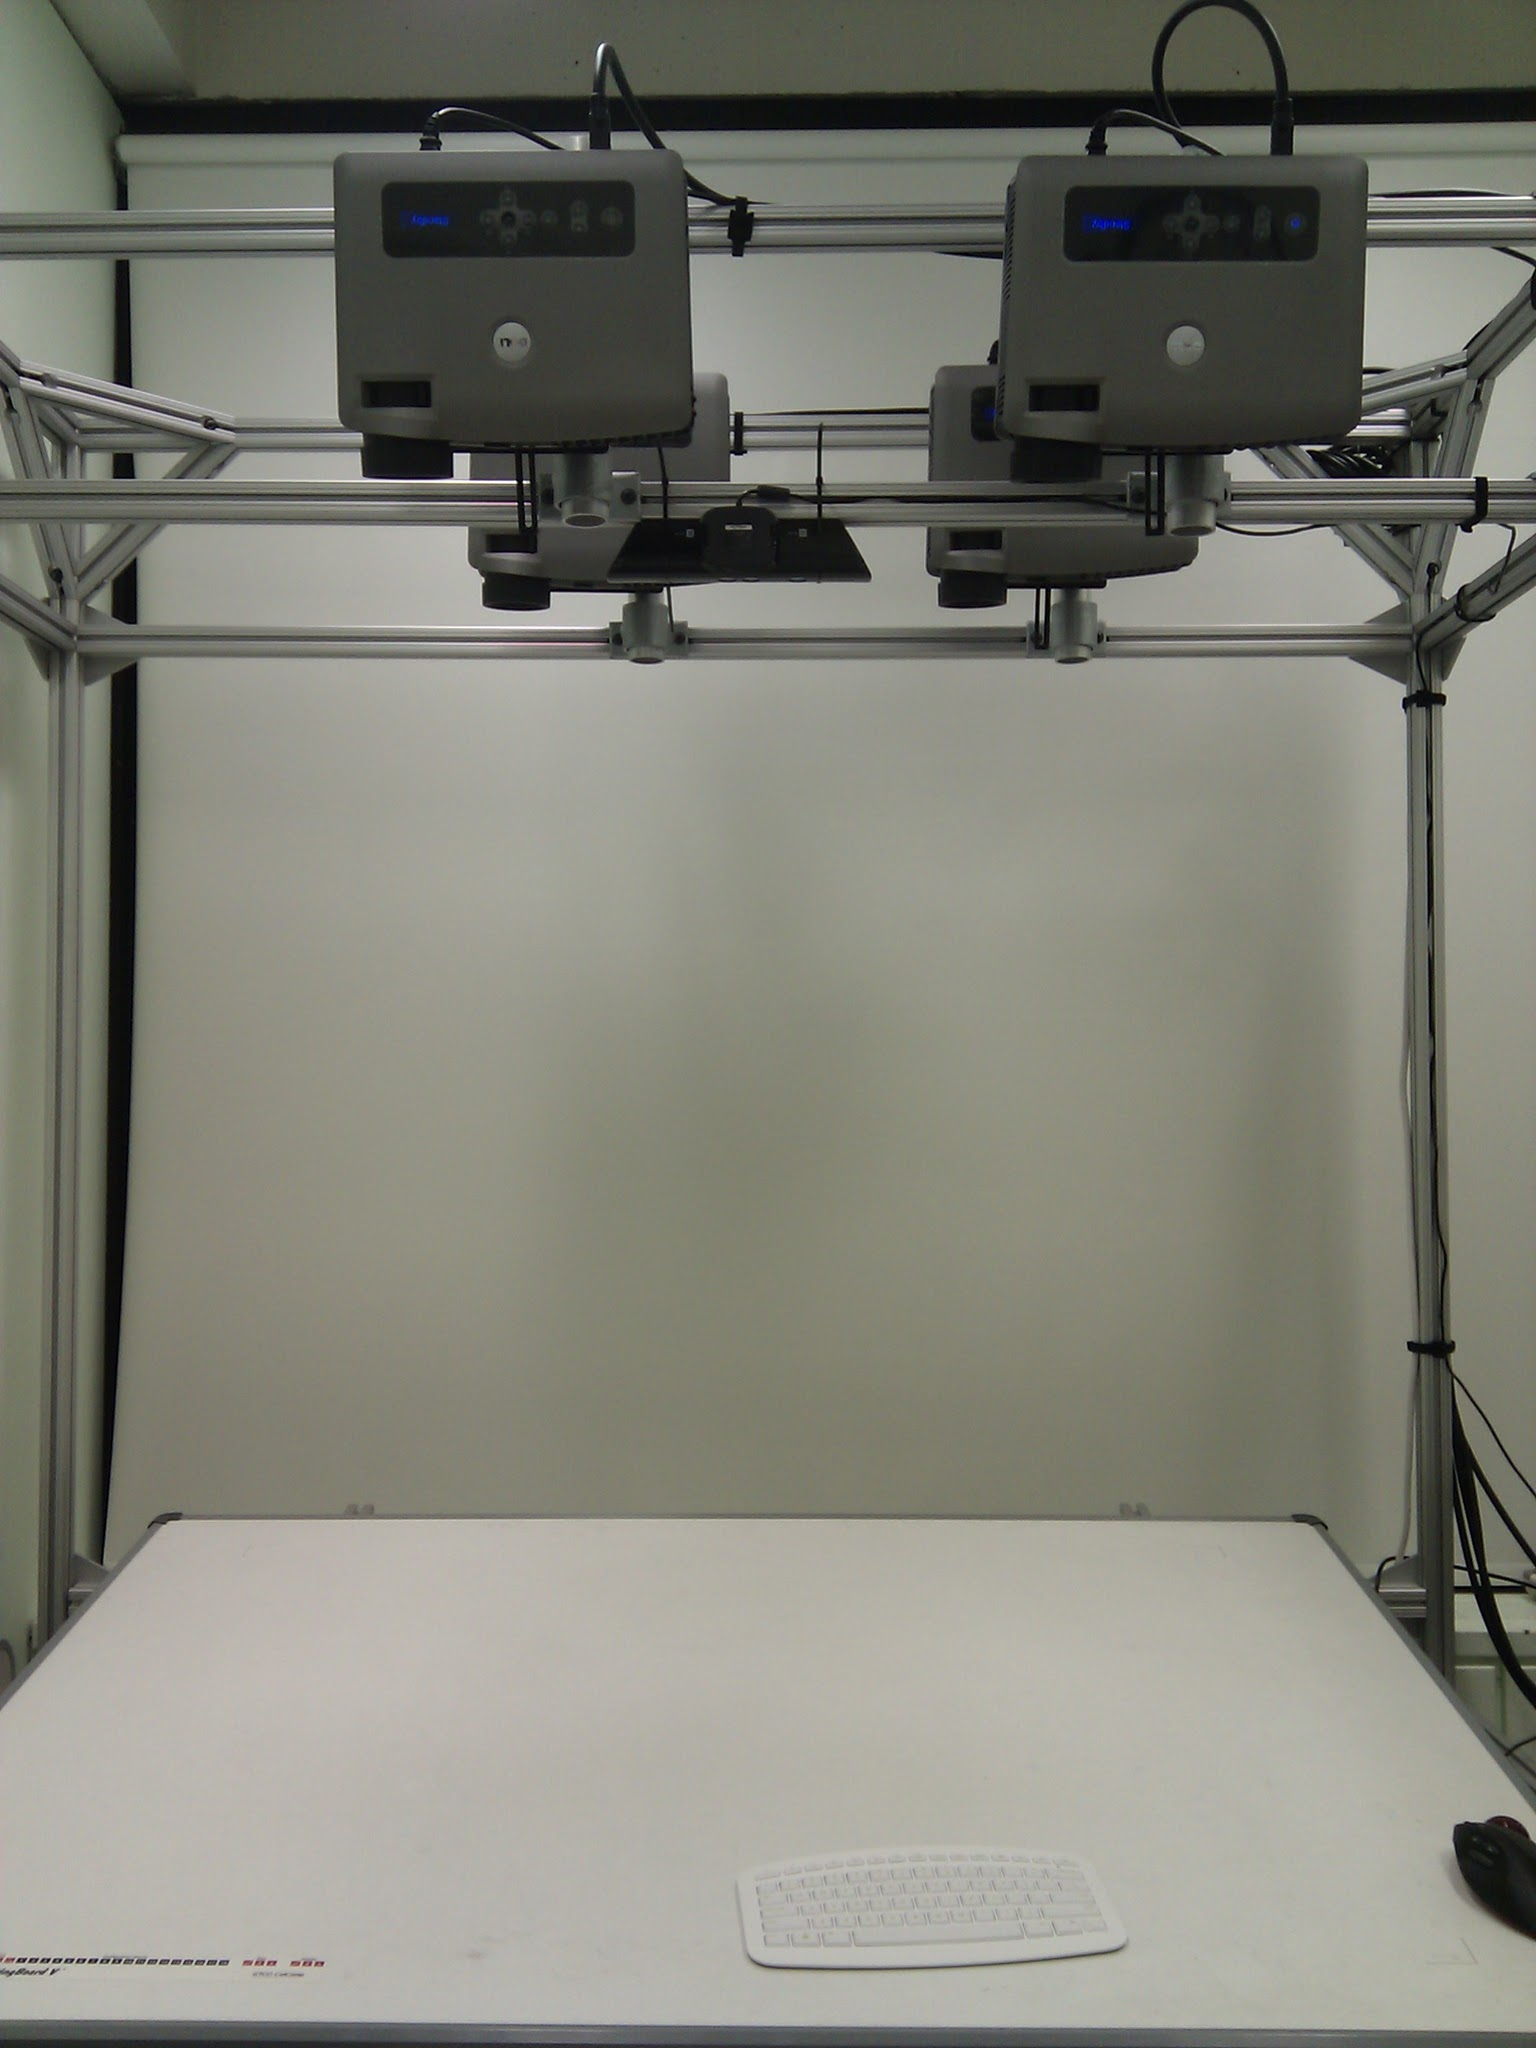
\includegraphics[width=0.4\textwidth]{figures/setup1.png} 
  }
  \subfigure[] {
  	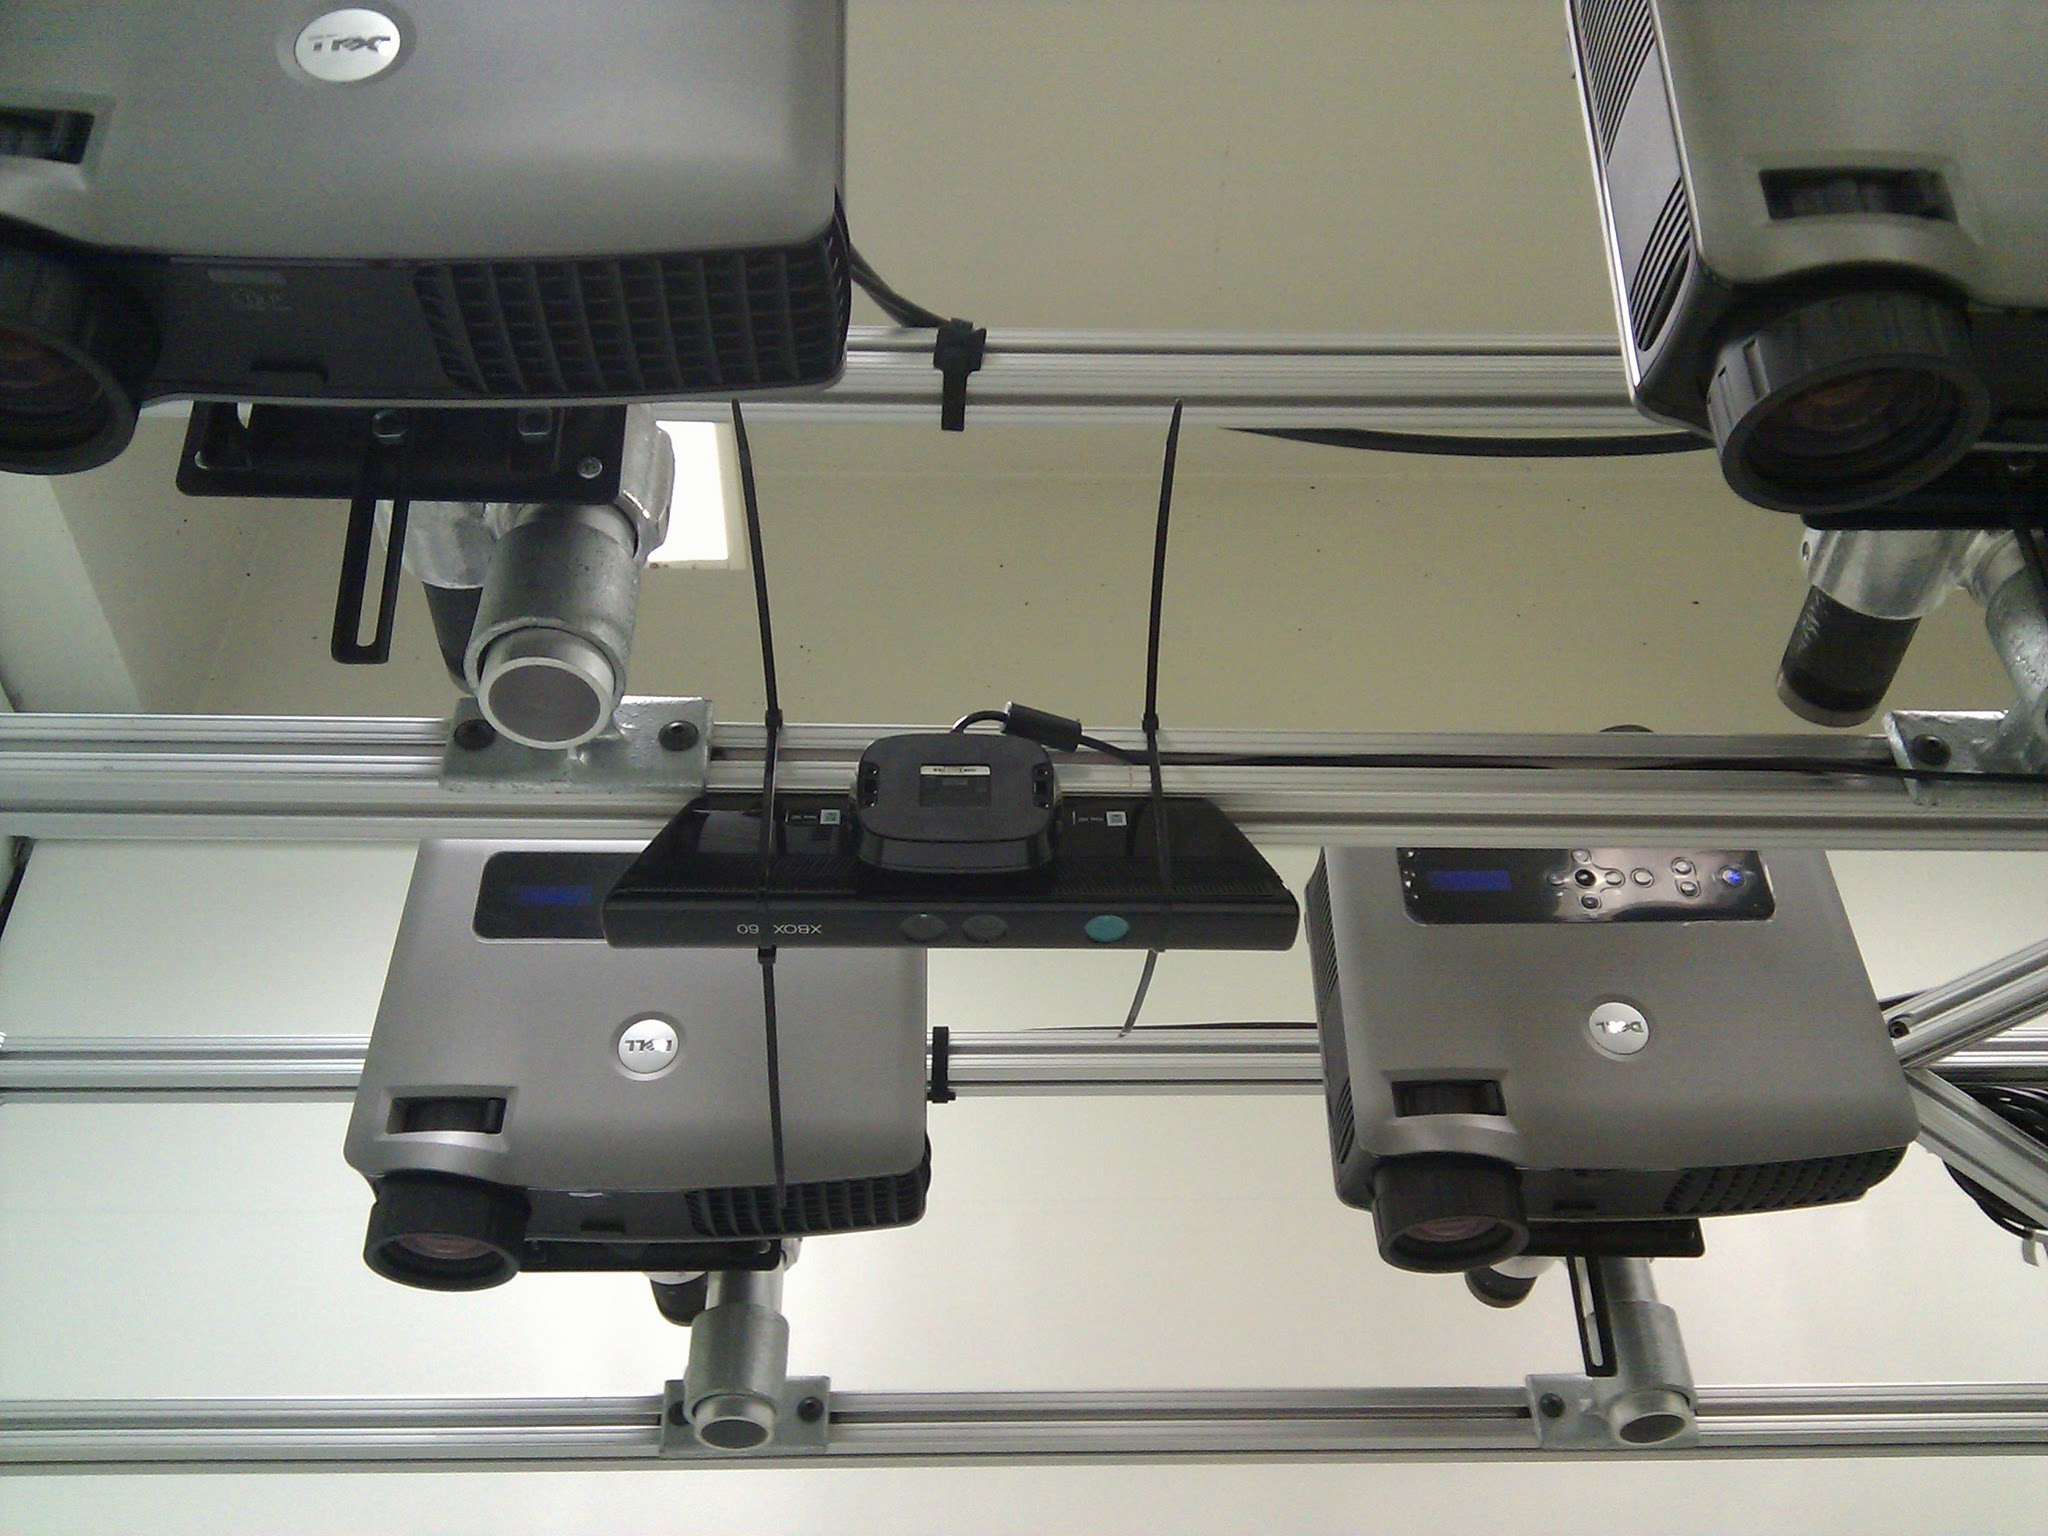
\includegraphics[width=0.4\textwidth]{figures/setup_close.png}
  }
  \caption{System setup.} \label{fig:setup}
\end{figure}

One Kinect motion sensor by Microsoft is placed above the center of the tabletop
at the same level of the projectors. Figure~\ref{fig:setup} shows the setup. The
Kinect sensor has a RGB camera, a depth sensor and a multi-array microphone.
We use the depth sensor to capture hand motion data because it is
less sensitive to the lighting condition. This is particularly useful for our
projection system. The Dell 5100MP projector uses a spinning color wheel to
modulate the image. This produces a visible artifact on the screen, referred to 
as the ``rainbow effect'', with colors separating out in distinct red, green, 
and blue. At any given instant in time, the image on the screen is either red, or green, or blue,
and the technology relies upon people's eyes not being able to detect the rapid 
changes from one to the other. However, when seen through a RGB camera, the
effect is very obvious, and this can greatly affect hand segmentation if we were to use 
the RGB images. 

The Kinect sensor outputs video at a frame rate of 30Hz. The depth sensing video
stream has a resolution of $640\times 480$ pixels with 11-bit depth value. The
depth value increases as the distance of the object from the sensor increases.
The depth sensor has a range limit of about 0.5m - 5m with a resolution of 1.5mm
at 0.5m and 5cm at 5m. The tabletop surface is about 1.2m away from the Kinect
sensor which allows us to have a relatively good depth resolution. We use the
open source OpenNI framework \footnote{https://github.com/OpenNI/OpenNI} and its
Kinect driver \footnote{https://github.com/avin2/SensorKinect} to get both the depth and RGB data streams.

\subsection{Kinect Calibration}
In order to develop an interactive interface, we need to map the point in the
depth image to the point on the display. We do this by projecting a
checkerboard image on the tabletop display, and placing some wooden blocks at
the corners of the checkerboard image to create the depth differences so that 
the depth sensor can capture these corners (see Figure~\ref{fig:calibration}).
We manually labeled 16 pairs of corresponding points on the display and the depth image. Then we
apply undistortion to the depth image and planar homography to find the mapping.

\begin{figure}[h]
  \centering
  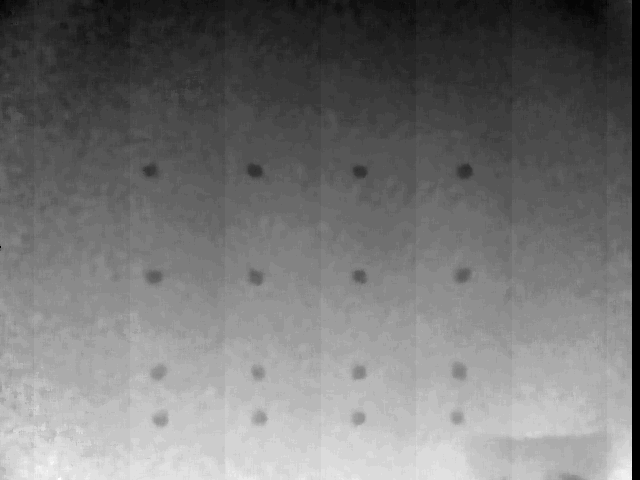
\includegraphics[width=0.5\textwidth]{figures/calibration.png} 
  \caption{Kinect calibration. The darker squares are the wooden blocks. The
  intensity of the gray level image is inversely proportional to the distance
  from the Kinect sensor.}
  \label{fig:calibration}
\end{figure}

Planar homography is a projective mapping from one plane to another. In our
case, we are mapping points on the plane of the depth image to the points
on the plane of the display. To evaluate the result of the calibration, we
obtain a new set of manually labeled corresponding points on the display and the
depth image. We then transform the coordinates of the points on the depth image
to the coordinates on the display using the calibration result, and find the
Euclean distance (error) between the transformed coordinates and the labeled
coordinates of the points on the display. The average errors in the x-axis and
y-axis are 4.3px and 8.9px respectively, which are 0.21cm, and 0.4cm in physical distance of the
projected display. The average width of the index fingertip is about 1.4cm, so
the error is less than 30\% of the width of the fingertip. 

\subsection{Hand Tracking}
The hand tracking process consists of feature detection and parameter estimation. The hand tracking
pipeline consists the following steps:

\begin{enumerate}
  \item Background subtraction
  \item Forelimb and hand segmentation
  \item Fingertips tracking
\end{enumerate}

The following subsections explain in details about these steps. Many of the
computer vision methods we use are based on the OpenCV
\footnote{http://opencv.willowgarage.com/wiki/} library and its Java interface 
JavaCV \footnote{http://code.google.com/p/javacv/}.

\subsubsection{Background Subtraction}
While the background - i.e., the tabletop - is relatively static, there is
still noise from the depth sensor. We use the averaging background method, which
learns the average and average difference of each pixel in the depth image as
the model of the background. The average values are based on the initial 30
frames with no hands in the scene. For the subsequent frames, any value that is 
6 times the average frame-to-frame absolute difference below the average tabletop depth value for that pixel is considered 
foreground because it is closer to the sensor above.

To clean up the background subtracted depth image, we use 1 iteration of
morphological opening to clear out small pixel noise. Morphological opening is a
combination of erosion and dilation. Both erosion and dilation are morphological
transformations. The kernel of erosion is a \textit{local minimum} operator,
while that of dilation is a \textit{local maximum} operator.

\begin{figure}[h]
  \centering
  \subfigure[Without using morphological opening.] {
	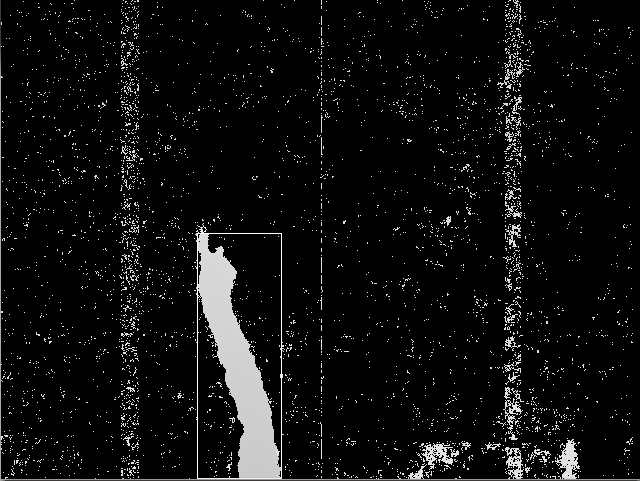
\includegraphics[width=0.4\textwidth]{figures/background_subtraction.png} 
  }
  \subfigure[Using morphological opening to clear out small pixel noise.] {
  	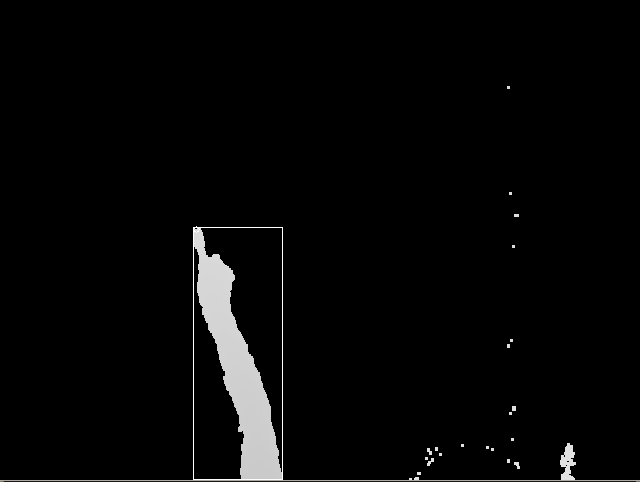
\includegraphics[width=0.4\textwidth]{figures/morphology.png}
  }
  \caption{Background subtraction.} \label{fig:setup}
\end{figure}


\subsubsection{Forelimb and Hand Segmentation}
With the cleaned up background subtracted depth image, we find connected
components by finding all contours that are not too small. These components are
considered to be the forelimbs and are approximated with convex hulls and 
bounding boxes. The hand region is at either end of the bounding box depending
on the position of the arm relative to the table.

\subsubsection{Fingertips Tracking}
We base our estimation of the hand model on geometric properties of the
hand. We compute the convexity defects from the convex hull of the forelimb
(Figure \ref{fig:convexity_defects}). From this we can observe that for an
extended finger, it has one convexity defect on each side and the two adjacent sides of the defects form an
acute angle. We iterate through the adjacent convexity defects, and mark the
intersection of those sides that form an angle smaller than a threshold
value as the potential fingertip. We further refine the fingertip position by
searching in the general direction of the finger and finding a sharp change in
the gradient of the depth value.

\begin{figure}[h]
  \centering
  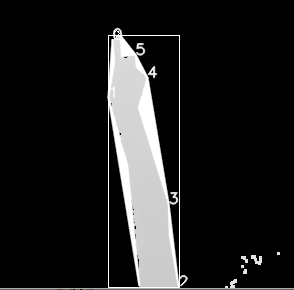
\includegraphics[width=0.4\textwidth]{figures/convexity_defects2.png} 
  \caption{The white triangles are the convexity defects.}
  \label{fig:convexity_defects}
\end{figure}

\subsubsection{Kalman Filter}
We use a Kalman filter to further improve tracking accuracy. The dynamic state
of the fingertip can be summarized by a $4$-dimensional vector, $x_k$, including
two position variables, $x$ and $y$, and two velocities, $v_x$ and $v_y$. The
measurement is a $2$-dimensional vector, $z_k$, of the measured $x$ and $y$ coordinates of the fingertip.

Assuming no external control, the a priori estimate $x_k^-$ of the state is
given by:
\begin{align*}
x_k^- = Fx_{k - 1} + w_k
\end{align*}
$F$ is the $4$-by-$4$ \textit{transfer matrix} characterizing the
dynamics of the system with the following values:

\begin{align*}
x_k = \begin{bmatrix}
	x   \\
	y   \\
	v_x \\
	v_y \end{bmatrix}_k, \quad
F = \begin{bmatrix}
	1 & 0 & 1 & 0 \\
	0 & 1 & 0 & 1 \\
	0 & 0 & 1 & 0 \\
	0 & 0 & 0 & 1 \end{bmatrix}
\end{align*}
assuming constant velocities, and that time is measured in frames.
$w_k$ is the \textit{process noise} associated with random events or forces
that directly affect the actual state of the system. We assume that the 
components of $w_k$ have Gaussian distribution $N(0, Q_k)$ for some $4$-by-$4$ 
covariance matrix $Q_k$. We set the matrix $Q$ with the following values:
\begin{align*}
Q = \begin{bmatrix}
	1 & 0 & 0 & 0 \\
	0 & 1 & 0 & 0 \\
	0 & 0 & 10 & 0 \\
	0 & 0 & 0 & 10 
	\end{bmatrix}
\end{align*}
The larger variance values indicate the greater uncertainty in the velocities as
they may not be constant.

\subsubsection{Evaluation}
We evaluate the accuracy of our fingertip tracking method by comparing the
detected fingertip position with the manually labeled position in a sequence of
video frames. In this first evaluation, only one extended finger is used. Our
method finds all the labeled fingertips and the average error (Euclean distance)
is 5.3px which is about 10mm. In their finger click evaluation, Harrison et al.
reports that their system has an average of 11.7mm offset from the targets. 

Here we want to emphasize that the focus of the thesis is gesture recognition
and finding a hand model that is suitable for gestural input. As a result, we
are not pushing the accuracy of fingertip and click detections to as high as
possible. We also envision that better touch screen hardware will be developed
in the near future with larger size and higher resolution, and hence, touch
detection accuracy can be very high. Our hand model and gesture analysis
framework should be general enough such that it can be easily adapted to
different sensor inputs.

The result of parameter estimation of the hand model is used both as the input
to the gesture recognizer and the system response to manipulative gestures. One
research question we want to investigate is what level of complexity of the
hand model is needed for the manipulative task. Do we need a 26 DOF skeleton
model, or would a simplified model with a smaller number of DOFs suffice?
Is tracking fingertips, or even just tracking the contact area of the hand for
surface gestures enough for the manipulative tasks?

\subsection{Hierarchical Approach to Real-Time Gestural Analysis}
As mentioned in Section \ref{sec:taxonomy}, we propose a systematic approach to
enabling gestural interaction according to the hierarchical taxonomy of
gestures. Unintentional movements should be ignored by the system.
Manipulative gestures require frame-by-frame tracking of the hand so that the
system can make real-time update to the virtual object being manipulated according to the hand
movement. Communicative gestures require system response after the user acts.

The research question here is how we can first differentiate the broader
categories of gestures, and then further classify the gestures into more 
specific categories. One possibility is to explore the inherent difference
between unintentional movements, manipulative gestures and communicative
gestures. For examples, manipulative gestures tend to be
slower, and have definite hand poses; some unintentional movements, like
``beats'', tend to be fast, repetitive, and close to the body. We can also
utilize the context constraints to narrow down the possibility of the gestures. For example, if the hand is at the position of a movable object, the probability
for it to be a manipulative gesture is higher. We can combine both the inherent
hand movement features and the context constraints to build a probabilistic
model to differentiate the broader categories of the hand movements.

The rationale for breaking down the hand movements according to the broader
categories is that the features that are relevant to each categories are
different. For manipulative gestures, we need to track the positions and 
orientation of the fingertips and the hand so that we can update the position 
and orientation of the virtual object being manipulated. For deictic gestures, 
we need to know the general pointing direction. For symbolic gestures, both the 
static hand poses and the dynamic hand movement need to be considered as 
features in the models. We propose that using different models for
different categories can improve the performance of the system. 

We combine different levels of recognition using the abstract hidden Markov
model (AHMM) architecture. The AHMM is a probabilistic model used to explain the
interaction between behaviors at different levels of abstraction \cite{johns05}.
It is also closely related to the hierarchical HMM (HHMM) \cite{fine98}. We can
map the levels in our gesture taxonomy into the levels of abstraction in an
AHMM. The higher abstract levels represent the mental intention of the gesturer.
We need to determine what is the optimal number of levels to use in AHMM. We can
use the number that resemble the hierarchy of our taxonomy. But the greater the 
number, the greater the computational complexity. A flatter model may be more 
reasonable and may not affect accuracy very much. The bottom level in the AHMM 
consists of observations and states in a typical HMM. An HMM is suitable for 
modeling sequential data such as time series, and has been used widely for 
dynamic gesture recognition with reasonable success. Kalman filter model is 
widely used for tracking objects. It can be viewed as a special case of HMM
where state transition probabilities and emission probabilities are all Gaussian. As 
a result, we propose to combine these two together under a unified framework of 
AHMM where a Kalman filter is used for tracking hands for manipulative gestures 
and HMMs are used for dynamic gesture recognition. We also treat static gesture 
as a special case of dynamic gesture with only one state.

We will start with a simple 1-level AHMMs \cite{murphy02} first (Figure
\ref{fig:amms}). $G_t$ represents the mental concept of the gesture that the
gesturer currently has. It includes unintentional movements ($U$), manipulative
gestures ($M$), and various communicative gestures ($C_i$). $S_t$ is the hidden
state of the hand pose and movement, which is essentially a vector quantization of the actual, observed 
(but noisy) feature vector $X_t$. $F_t^G$ is a binary indicator variable that is
``on'' (has value 1) if the lower level HMM at time $t$ has just ``finished''
(i.e., is about to enter an end state), otherwise it is ``off'' (has value 0).

\tikzstyle{vertex}=[circle, draw, minimum size=16pt, inner sep=0pt]
\tikzstyle{observed-vertex}=[circle, draw, minimum size=16pt, inner sep=0pt,
							 fill=black!20] 
\tikzstyle{edge} = [draw, thick, -]
\tikzstyle{directed-edge} = [draw, thick, ->]

\begin{figure}[h]
\centering
  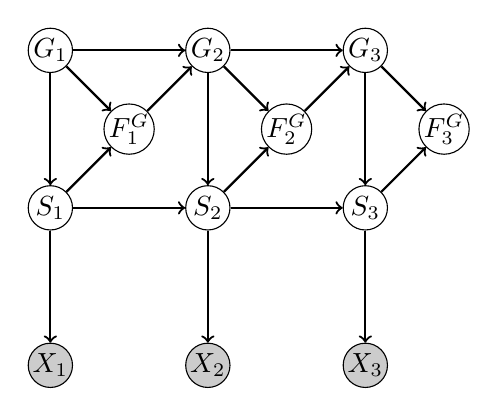
\begin{tikzpicture}[auto,swap, scale=2]
    % First we draw the vertices
    \foreach \pos/\name in {{(0, 2)/G_1}, {(1, 2)/G_2}, {(2,2)/G_3},
    	{(0.5,1.5)/F_1^G}, {(1.5,1.5)/F_2^G}, {(2.5, 1.5)/F_3^G},
    	{(0, 1)/S_1}, {(1, 1)/S_2}, {(2, 1)/S_3}} 
      \node[vertex] (\name) at \pos {$\name$};
    \foreach \pos/\name in {{(0, 0)/X_1}, {(1, 0)/X_2}, {(2, 0)/X_3}}
      \node[observed-vertex] (\name) at \pos {$\name$};
    % Connect vertices with edges and draw weights
    \foreach \source/ \dest in {G_1/S_1, S_1/X_1, G_1/F_1^G, S_1/F_1^G,
    							F_1^G/G_2, G_1/G_2, G_2/S_2, S_2/X_2, G_2/F_2^G,
    							S_2/F_2^G, F_2^G/G_3, G_2/G_3, G_3/S_3, S_3/X_3,
    							G_3/F_3^G, S_3/F_3^G, S_1/S_2, S_2/S_3} 
      \path[directed-edge] (\source) -- (\dest);
  \end{tikzpicture}
  \caption{A 1-level AHMM. $F_t^G$ turns on if state $S_t$ satisfies goal
  $G_t$; this causes a new goal to be chosen. However, the new state may depend
  on the old state; hence there is no arc from $F_{t-1}^G$ to $S_t$ to
  ``reset'' the submodel \cite{murphy02}.}
  \label{fig:amms}
\end{figure}

\subsection{Discriminative Training}
HMMs as a generative model allows us to model the joint
distribution of the observed sequence. Traditionally,
maximum-likelihood (ML) estimation is used to learn the parameters of HMMs. However, our real task is to
classify the sequence of the observed data. Discriminative classifiers model the
posterior $p(y|x)$ directly, and hence are believed to give a lower error rate.
In the speech recognition community, discriminative training methods have been
proposed and have shown significant improvements over ML-trained models on many
large vocabulary speech recognition tasks \cite {chang12}. To further improve
the discriminative power of our model, we will use discriminative training
methods for gestural analysis.

HMM provides a computationally efficient modeling framework. The HMM makes two
main assumptions:

1. There exists a hidden state sequence, $S$, that forms a Markov chain that
generates the observation vectors.

2. Given the state $s_t$ at any time point, the corresponding observation $x_t$
is conditionally independent of other observations and states.

Instead of seeking model parameters that can maximize the likelihood of the
data, discriminative training methods seek parameters that can minimize the
confusions that occur in the training data. In general, discriminative training
methods consist of two steps: First, construct a smooth and efficient computable
objective function that reflects the degree of confusion; second, adjust the
model parameters such that the objective function can be optimized. 

We will explore several commonly used discriminative training criteria such as
minimum classification error training, maximum mutual
information training, and margin-based training methods. For optimizing
parameters, we can use either the extended Baum-Welch method or gradient-based
methods. We will also compare the results to those without discriminative
training and those with CRF-based models.

\subsection{Gesture Spotting}
\textit{Gesture spotting} is a method that
distinguishes meaningful gestures from unintentional movements \cite{kang04}.
Hand movements are signified by motion. We can detect the start and the end of a hand movement by the amount of motion. This forms a segment
which is a candidate hand movement. 

Instead of using hard coded threshold values for detecting candidate
start and end frame as in \cite{kang04}, we will use machine learning methods to
make the result more robust. We propose to use a support vector machine (SVM) to
classify each frame into either a candidate start, candidate end or neither. One
important question here is what features we should use for the feature vector.
We will experiment with the criteria used in \cite{kang04} which are motion
energy, static poses, and curvature, and will also explore other possible
features such as positions relative to the body or table, and accompanying
speech etc.

In order to combine the result of the SVM with our probabilistic model, we use
the probabilistic output from SVM as proposed by Platt \cite{platt99}.

\subsection{Multi-modal Interaction with Gesture and Speech} 
For this thesis, we focus on gestural input and interaction. However, we will
also add some basic speech recognition capability to combine speech and gestures
for some USAR interaction scenarios. We will use an off-the-shelf speech 
recognizer, and investigate how to combine both speech and gesture to make
the interaction more natural and effortless. Specifically, we will explore the
alignment of speech and gesture, mutual disambiguation of speech and gesture,
and how speech and gestures complement each other in certain scenarios.

\subsection{Motivating Application}
We will develop a simple game-like application that simulates some of the USAR
interaction scenarios. The game will be browser-based for easy access. With the
recent development in HTML5, browser-based interaction becomes richer and
richer. Web browsers have become the main application people use to do various
tasks because they provide better accessibility to information via the
Internet. We believe that being able to use gesture as an input to the browser
will make a big contribution to HCI as well.

The game we have in mind is highly inspired by
StarCraft\footnote{http://us.battle.net/sc2/en/}. StarCraft is a real-time
strategic game that involves controlling different kinds of units to accomplish
a vast array of tasks. The game's richness in command and control can help us develop a set of gestural language in this domain.

The gestural input functionality we want demonstrate in this application are:

\begin{enumerate}
  \item Moving units from one location to another
  \item Panning the map
  \item Command a unit to build different kinds of buildings, like recycler,
  barrack, and factory etc.
  \item Command units to attack the enemies by doing an attack gesture (say
  ``attack'') and pointing to the location of attack
\end{enumerate}

\subsection{User Study}\label{sec:user_study}
We will bootstrap the system with a set of natural gestures defined based on the
user studies done by Yin et al. \cite{yin10} and Wobbrock et al.
\cite{wobbrock09} on the set of natural gestures people do for surface
computing. We will conduct a user study after making a simple application where
the user can perform both manipulative and communicative gestures. The goal of 
the user study is to evaluate the accuracy of the hand tracking and gesture 
recognition. A research question here is whether we can bootstrap the system 
only with the gesture examples we provide ourselves, or we need to collect 
training examples from the users, and how well the system performs 
independent of users.

\section{Schedule}
\begin{enumerate}
  \item Improve fingertips tracking \hfill Done by April 30, 2012

  Improve the Kalman filter method by adjusting the noise covariance matrix
  based on the confidence of the feature extraction. Finish multiple fingertips
  tracking and quantitative evaluation of the tracking accuracy.
  
  \item Improve fingertip touch detection \hfill Done by May 15, 2012
  
  Finish quantitative evaluation of click detection (fingertip touching the
  table surface). The true positive (detecting a click when there is a click
  event) rate should be at least 96.5\% (comparable with the number reported in
  \cite{harrison11}, but our method has fewer constraints on the position of users' hands). The false positive rate should
  be less than 2.6\%. The false negative rate should be less than 0.8\%.

  \item Detection of start and end of gestures \hfill Done by May 28, 2012

  \item Model unintentional gestures \hfill Done by Oct 01, 2012

  \item Develop AHMMs framework	\hfill Done by Jan 01, 2013

  Develop the AHMMs hierarchical model and combine the model for start and
  end of hand movements, the model for unintentional movement and HMM models for
  communicative gestures. 
  
  \item Discriminative training and evaluation \hfill Done by Mar 01, 2013
  
  \item Develop browser-based game application \hfill Done by May 01, 2013
    
  \item Combine speech with gesture	\hfill Done by Jun 01, 2013

  \item User study \hfill Done by Jul 01, 2013

  Conduct user study described in Section \ref{sec:user_study}.
  
  \item Write the first draft of thesis report \hfill Done by Sep 01, 2013
  \item Complete thesis report	\hfill Done by Oct 01, 2013
  \end{enumerate}

\section{Principal Equipment and Facilities}
Here is a list of equipment and facilities needed for the study:

\begin{enumerate}
  \item A white surface digitizer (GTCO Calcomp DrawingBoard V)
  \item Four $1280\times1024$ pixel projectors (Dell 5100MP)
  \item One Kinect motion sensor
  \item One desktop with a powerful graphics card (1GB memory, at least 4 ports)
\end{enumerate}

All the above equipment is available.

\section{Appendix A - Review of Kalman Filter}
Let $x_k$ be an $n$-dimensional vector of state components and $P_k$ be the
$n$-by-$n$ error covariance. The measurement $z_k$ is an $m$-dimensional
vector given by:
\begin{align*}
z_k = H_kx_k + v_k,
\end{align*}
where $H_k$ is an $m$-by-$n$ matrix and $v_k$ is the measurement error.

The \textit{Kalman gain}, $K_k$, is an $n$-by-$m$ matrix expressed as:
\begin{align*}
K_k = P_k^-H_k^T(H_kP_k^-H_k^T + R_k)^{-1}
\end{align*}

Assuming no external control, the a priori estimate $x_k^-$ of the state is
given by:
\begin{align*}
x_k^- = Fx_{k - 1} + w_k,
\end{align*}
where $F$ is the $n$-by-$n$ \textit{transfer matrix} characterizing the
dynamics of the system, and $w_k$ is the \textit{process noise} associated with
random events or forces that directly affect the actual state of the system. We assume that the components of $w_k$
have Gaussian distribution $N(0, Q_k)$ for some $n$-by-$n$ covariance matrix
$Q_k$.

Using $P_k^-$ to denote the error covariance, the a priori estimate for this
covariance at time $k$ is obtained from the value at time $k - 1$ by:
\begin{align*}
P_k^- = FP_{k - 1}F^T + Q_{k - 1}
\end{align*}

The updated value for $x_k$ when a new measurement is available is:
\begin{align*}
x_k = x_k^- + K_k(z_k^- - H_kx_k^-)
\end{align*}
The update value for $P_k$ is:
\begin{align*}
P_k = (I - K_kH_k)P_k^-
\end{align*}

\section{Appendix B - Review of Dynamic Bayesian Network}
This part is mainly based on the Ph.D. thesis by Murphy \cite{murphy02}.

An HMM is a stochastic finite automaton, where each state generates (emits) an
observation. If we let $S_t$ represent the hidden state at time $t$, the
transition model between states can be characterized by a conditional
multinomial distribution: $A(i, j) = P(S_t = j | S_{t-1} = i)$, where $A$ is a
stochastic matrix.

\subsection{Filtering}
The most common inference problem in online analysis is to recursively estimate
the belief state using Bayes's rule:

\begin{align*}
P(S_t | x_{1:t}) & \propto P(x_t | S_t, x_{1:t-1})P(S_t | x_{1:t-1}) \\
 				 & = P(x_t | S_t) \left[\sum_{s_{t - 1}} 
				 	 P(S_t | s_{t - 1})P(s_{t - 1} | x_{1:t - 1})\right]	
\end{align*}

This task is traditionally called ``filtering'', because we are filtering out
the noise from the observations. We can find this value using the forward
algorithm.

\subsection{Classification}
The likelihood of a model, $M$, is $P(x_{1:t}|M)$. This can be used to classify
a sequence as follows:
\begin{align*}
C^*(x_{1:T}) = \arg \max_{C} P(x_{1:T} | C)P(C)
\end{align*}

\section{Appendix C - Review of Random Conditional Fields}
Each clique template $C_p$ is a set of factors which has a corresponding set
of sufficient statistics $\{f_{pk}(\mathbf{x_p}, \mathbf{y}_p)\}$ and
parameters $\theta_p\in\mathcal{R}^{K(p)}$. The CRF can be written as
\begin{align}
p(\mathbf{y}|\mathbf{x}) = \frac{1}{Z(\mathbf{x})}\prod_{C_p\in
\mathcal{C}}\prod_{\Psi_c\in C_p}\Psi_c(\mathbf{x}_c,
\mathbf{y}_c;\theta_p)
\end{align}
where each factor is parameterized as
\begin{align}
\Psi_c(\mathbf{x}_c, \mathbf{y}_c;\theta_p) =
\exp\left\{\sum_{k=1}^{K(p)}\lambda_{pk}f_{pk}(\mathbf{x}_c,
\mathbf{y}_c)\right\}
\end{align}
and the normalization function is 
\begin{align}
Z(\mathbf{x}) 
&= \sum_{\mathbf{y}}\prod_{C_p\in\mathcal{C}}\prod_{\Psi_c\in
C_p}\Psi_c(\mathbf{x_c}, \mathbf{y_c}; \theta_p)\\
&= \sum_{\mathbf{y}}\exp\left\{\sum_{C_p\in\mathcal{C}}\sum_{\Psi_c\in
C_p}\sum_{k=1}^{K(p)}\lambda_{pk}f_{pk}(\mathbf{x}_c,
\mathbf{y}_c)\right\}
\end{align}

The conditional log likelihood is given by 
\begin{align}
\ell(\theta) = \sum_{C_p\in\mathcal{C}}\sum_{\Psi_c\in
C_p}\sum_{k=1}^{K(p)}\lambda_{pk}f_{pk}(\mathbf{x}_c, \mathbf{y}_c) - \log Z(\mathbf{x})
\end{align}

The partial derivative of the log likelihood with respect to a parameter
$\lambda_{pk}$ associated with a clique template $C_p$ is
\begin{align}
\frac{\partial\ell}{\partial\lambda_{pk}} 
&= \sum_{\Psi_c\in C_p}\lambda_{pk}f_{pk}(\mathbf{x}_c, \mathbf{y}_c) -
\frac{1}{Z(\mathbf{x})}\frac{\partial Z(\mathbf{x})}{\partial\lambda_{pk}}\\
&= \sum_{\Psi_c\in C_p}\lambda_{pk}f_{pk}(\mathbf{x}_c, \mathbf{y}_c) -
\frac{1}{Z(\mathbf{x})}\sum_{\mathbf{y}}\exp\left\{\sum_{C_p\in\mathcal{C}}\sum_{\Psi_c\in
C_p}\sum_{k=1}^{K(p)}\lambda_{pk}f_{pk}(\mathbf{x}_c,
\mathbf{y}_c)\right\}\sum_{\Psi_c\in C_p}f_{pk}(\mathbf{x}_c, \mathbf{y}_c) \\
&= \sum_{\Psi_c\in C_p}\lambda_{pk}f_{pk}(\mathbf{x}_c, \mathbf{y}_c) -
\frac{1}{Z(\mathbf{x})}\sum_{\mathbf{y}}p(\mathbf{y}, \mathbf{x})\sum_{\Psi_c\in
C_p}f_{pk}(\mathbf{x}_c, \mathbf{y}_c) \\
&= \sum_{\Psi_c\in C_p}\lambda_{pk}f_{pk}(\mathbf{x}_c, \mathbf{y}_c) -
\frac{1}{Z(\mathbf{x})}\sum_{\Psi_c\in C_p}\sum_{\mathbf{y}}p(\mathbf{y},
\mathbf{x})f_{pk}(\mathbf{x}_c, \mathbf{y}_c) \\
&= \sum_{\Psi_c\in C_p}\lambda_{pk}f_{pk}(\mathbf{x}_c, \mathbf{y}_c) -
\frac{1}{Z(\mathbf{x})}\sum_{\Psi_c\in C_p}\sum_{\mathbf{y'_c}}p(\mathbf{y'_c},
\mathbf{x})f_{pk}(\mathbf{x}_c, \mathbf{y'}_c) \\
&= \sum_{\Psi_c\in C_p}\lambda_{pk}f_{pk}(\mathbf{x}_c, \mathbf{y}_c) -
\sum_{\Psi_c\in C_p}\sum_{\mathbf{y'_c}}f_{pk}(\mathbf{x}_c, \mathbf{y}_c)p(\mathbf{y'_c}
| \mathbf{x})
\end{align}

\section{Appendix D - Online Inference}


